\chapter{Introduction}\label{ch:introduction}
% \TODO{
% \begin{enumerate}
%     \item CBT-UA -> UA-CBT everywhere
% \end{enumerate}

% }
% \epigraph{Нації вмирають не від інфаркту. Спочатку їм відбирає мову.
% \\ 
% \textit{Nations don\textquotesingle t die from heart attacks. They go mute first.}}{Ліна Костенко \\ Lina Kostenko, Ukrainian poetess}

% \epigraphhead[10pt]{
% \epigraph{"evals are surprisingly often all you need"}{
% Greg Brockman, OpenAI President
% \footnote{\href{https://twitter.com/gdb/status/1733553161884127435}{Greg Brockman on X: "evals are surprisingly often all you need" / X}}
% }
% }

% The Ukrainian language is not at risk of dying, and as of 2023, this
% much is certain. But before 2014, the quote above was so incisive it
% \emph{hurt}.

\section{Motivation and summarized contributions}
\subsection{Motivation}
The last 10 years have seen a resurgence of the Ukrainian language,
especially its use in informal and non-academic contexts, with especially sharp changes occurring since 24 February 2022.
This increase can be seen both in opinion polls and in statistics based on Twitter data (\autoref{the-contemporary-ukrainian-linguistic-landscape}).

The topic of mid– and low–resource languages was the focus of much discussion in recent years~\cite{inclusion}, and the support of under-resourced languages aligns with the broader objectives of computational linguistics (which studies \textit{language}, not English language).

In the case of Ukrainian, its increasing presence in the digital sphere is an additional indicator of a practical need for better Ukrainian support, with e.g. accurate machine translation, sentiment analysis, and information retrieval having the potential to impact the lives of many. 
(Though bad automated Russian-to-Ukrainian machine translation by malicious actors did have an unforgettable effect on Ukrainian popular culture as well~\cite{faichuk2023war}.)

On a 2020 survey~\cite{inclusion} on linguistic diversity in NLP, the
Ukrainian language was classed under ``rising stars'': languages with a
thriving community online, benefiting from pre-training on unlabeled data, but let down by insufficient \textit{labeled} data.
%A recent overview\cite{lai_chatgpt_2023} of the performance of LLMs on different languages found that it's quite uneven — ChatGPT performs best in English.

\subsection{Contributions}
This Thesis introduces Eval-UA-tion, the first Ukrainian-language LLM benchmark, and as
part of it introduces nine novel labeled datasets: 
\begin{enumerate}
    \item \textbf{UA-CBT}: A fill-in-the-blanks dataset based on novel children's stories generated by LLMs (and manually corrected afterwards), where one word is masked, and the task is to choose the correct word out of 6 options. The intent behind the task is to maximally force the LLM to understand the story narrative to make a correct choice. \\
    For example:\footnote{A complex example, most instances in the datasets are easier to solve.} \enquote{\textit{[...] The Merchant was sad to hear about the \textbf{\_\_\_\_}'s death}. 
 Options: a)~Hunter, b)~Wolf, c)~Bear.} 
 To answer correctly, the needed context is: 
 1)~both the Hunter and the Wolf are dead, but the Bear is still alive; 
 2)~the Merchant hired the Hunter to kill the Wolf, so he would not be sad about the Wolf's death.
    \item \textbf{LMentry-static-UA (LMES)}: A set of 6 tasks easy for humans but surprisingly hard for LLMs. 
    % \\ 
    For example: 
    \enquote{What is the first/third/last letter of the word `cactus'? Which word is longer, `cactus' or `dromedary'? 
    Which word doesn't belong to the category `emotions': sadness, happiness, depression, fear,  or pizza?}
    \item \textbf{UP-Titles}: Matching the correct article text to the correct title, out of a set of 10 similar titles. The dataset was created in two versions: one with all the digits masked (replaced by `X'), and one unchanged. The intent of the masked dataset is to increase the difficulty of the task by removing unique numbers whose presence both in the article text and one of the titles would provide a clue 
    (e.g. if the article contains the number 231 and one of the titles also does, it's likely the correct one)
\end{enumerate}

Random and human baselines were calculated for these datasets, followed by benchmarking a number of commercial and open LLMs (including GPT-3 and GPT-4).

\section{Research objectives}
\label{sec:research-objectives}
\begin{enumerate}
\tightlist
\item Analyze the currently available labeled datasets in Ukrainian language usable for the purposes of dataset benchmarking, to estimate the objective need for additional resources in that area. Analyze the existing NLP tools (e.g. morphology analyzers) and resources (e.g. corpora or dictionaries) usable for the dataset creation; and identify gaps.

\item How effective are the current LLMs at understanding and generating Ukrainian text, compared to human performance? Which areas present the most difficulties?

\item With the help of the newly created datasets, analyze whether Ukrainian-language fine-tuning increases the performance of Language Models on tasks involving the Ukrainian language.


\item By evaluating both commercial LLM solutions (e.g. OpenAI GPT-3 and GPT-4) and open-weights models, estimate to which extent smaller models with fewer parameters but with appropriate fine-tuning can be used for Ukrainian-language tasks instead of the much larger models.

\end{enumerate}


\section{Historical context and bilingualism in the modern Ukrainian
language}\label{historical-context}

\begin{quote}
\emph{L'Ukraine a toujours aspiré à être libre}\\
``Ukraine has always aspired to be free.'' \\ Voltaire, \href{https://books.google.com.ua/books?id=Lh8TAAAAQAAJ&pg=PA275&lpg=PA275&dq=\%22L\%E2\%80\%99Ukraine+a+toujours+aspir\%C3\%A9+\%C3\%A0+\%C3\%AAtre+libre\%22&source=bl&ots=gvCwzOT0nI&sig=ACfU3U2PCd60vC7uxL9hCteT47A0Iiq8og&hl=en&sa=X&ved=2ahUKEwjjuNuwqOb0AhUhpIsKHeHsCQcQ6AF6BAgUEAM\#v=onepage&q=\%22L\%E2\%80\%99Ukraine\%20a\%20toujours\%20aspir\%C3\%A9\%20\%C3\%A0\%20\%C3\%AAtre\%20libre\%22&f=false}{1731}\footnote{Voltaire, History of Charles XII, King of Sweden (1731)
~\cite{1817oeuvres}}
\end{quote}
% \footnote{\textbf{TODO}
%   format citation
%   \href{https://www.atlanticcouncil.org/blogs/ukrainealert/debunking-the-myth-of-a-divided-ukraine/}{Debunking
%   the myth of a divided Ukraine - Atlantic Council} citing
%   \href{https://books.google.com.ua/books?id=Lh8TAAAAQAAJ&pg=PA275&lpg=PA275&dq=\%22L\%E2\%80\%99Ukraine+a+toujours+aspir\%C3\%A9+\%C3\%A0+\%C3\%AAtre+libre\%22&source=bl&ots=gvCwzOT0nI&sig=ACfU3U2PCd60vC7uxL9hCteT47A0Iiq8og&hl=en&sa=X&ved=2ahUKEwjjuNuwqOb0AhUhpIsKHeHsCQcQ6AF6BAgUEAM\#v=onepage&q=\%22L\%E2\%80\%99Ukraine\%20a\%20toujours\%20aspir\%C3\%A9\%20\%C3\%A0\%20\%C3\%AAtre\%20libre\%22&f=false}{Oeuvres
%   complètes de Voltaire - Voltaire - Google Books}}

A significant number of people in Ukraine are bilingual (Ukrainian and
Russian languages), and most Ukrainians can understand both Russian and
Ukrainian~\cite{kulyk2018shedding}. 
The reasons for this include Ukraine\textquotesingle s geographical and
cultural proximity to Russia, as well as consistent policy (first of
the Russian Empire, then of the Soviet Union).
This section sketches the history of the language, describes the
bilingual nature of Ukraine\textquotesingle s society and the impact of
historical state policies on its modern development.

% The ongoing Russian invasion is viewed by many Ukrainians as a continuation of a
% long-standing historical pattern, rather than an isolated incident. 
% This
% section doesn\textquotesingle t attempt to justify or challenge any
% particular position regarding the events described, nor is meant to be a
% definitive account. 
The perspective is important to contextualize 
the need for Ukrainian NLP as part of linguistic and cultural reclamation
of the distinct cultural identity Ukraine fought (and is fighting) 
to preserve. 

This identity is a digital identity as well — and one that is growing.
One role of Ukrainian NLP (and Ukrainian NLP resources) is in contributing
towards it, especially with the rising use of LLMs in everyday life.
Many people are using Ukrainian, but there is a limited amount of 
tooling and NLP resources to support that. 
A better support for Ukrainian is rarely a priority, 
with many instances where where Ukrainian (language, culture, identity, ...) 
is subsumed under (or mistaken for) the Russian (both in everyday life and 
as translated into priorities and biases). 

A deeper dive into the reasons for the latter is helpful to understand
the need for stronger support for Ukrainian NLP, and of the feelings
caused by e.g. having to fall back 
to Russian to solve issues (including when communicating with an LLM), which is a typical 
occurrence for many Ukrainians.%

% The rest of this section describes some of the complexities relating to the Ukrainian language, past and present, placing the need for Ukrainian NLP in a broader context.

% the current linguistic landscape in Ukraine, as well as
% the linguistic challenges and phenomena that had a direct relevance on
% this Thesis (LLMs switching to Russian, worse support for Ukrainian 
% in Python libraries, and similar).

% The rest of this section describes some of the complexities relating to the Ukrainian language, past and present, placing the need for Ukrainian NLP in a broader context. 

\subsection{Overview}\label{intro-todo-better-title}

The Ukrainian language belongs to the Slavic family of the Indo-European
languages (which also includes Polish, Czech, Serbian,
Bulgarian), specifically to its East Slavic branch, which contains
Belarusian, Russian, and Ukrainian~\cite{grenoble2010contact}. Towards
the end of the 10th century the East 
% Slavonic 
Slavic
group of dialects was
relatively uniform, with the differences separating Ukrainian, Russian
and Belarusian appearing since then, as the result of linguistic and
political processes~\cite{press2015ukrainian}.

While all three languages are mutually intelligible to a certain extent,%
\footnote{
One interesting aspect is the asymmetry in language intelligibility between
Russian and Ukrainian:
Ukrainians are ``clearly more successful'' in understanding Russians
than vice versa \cite{rehbein2014check}. This disparity suggests that factors beyond linguistic similarity are at play.
} 
Ukrainian
has more in common with Belarusian than with Russian
\cite{press2015ukrainian}; outside the branch, Ukrainian has partial
intelligibility with Polish~\cite{rehbein2014check}. 

\subsection{A short history of the Ukrainian language}
\label{sec:ukr-lang-history}
% \subsection{The suppression of Ukrainian in the Russian
% Empire}\label{the-suppression-of-ukrainian-in-the-russian-empire}
This stems from the fact that in the 15th century, parts of what is now
Ukraine and Belarus were part of the Polish-Lithuanian Commonwealth,
with Polish becoming the \emph{lingua franca} of Ukrainian-Belarusian
lands.
As a result, a large proportion of the Ukrainian lexicon consists of
borrowings from the Polish language, and vocabulary remains the
language component where the difference with Russian is most
immediately noticeable~\cite{press2015ukrainian}.

In the Russian Empire, the broader imperial ideology sought to
assimilate various ethnicities into a single Russian identity (with
Russian as the dominant language), and policies aimed at diminishing
Ukrainian national self-consciousness were a facet of
that~\cite{doi:10.1016/j.euras.2014.05.005}.
Ukrainian (then officially called \emph{little Russian}~\cite{press2015ukrainian} and considered a dialect) was
%\footnote{among many Russians and some Europeans it 'still is' according to the source document
  % \cite{doi:10.1016/j.euras.2014.05.005}
  % }
 stigmatized as a peasants' dialect of Russian,
%, with its literature not taken seriously; 
the general attitude being that
% "backward Ukrainians" 
Ukrainians needed to be ``civilized'' by Russia, by its
language and developed culture~\cite{doi:10.1016/j.euras.2014.05.005}.

Attempts to extinguish a separate Ukrainian identity
weren\textquotesingle t limited by stigmatization --- the history of
Ukrainian language bans is long enough to merit a separate Wikipedia
article, with the more notable ones
% in the Russian Empire 
being the 1863 \emph{Valuev Circular}~\cite{dibrova2017valuev}
(forbidding the use of Ukrainian in religious and educational printed
literature)\footnote{Also memorably stating that ``a separate Little
  Russian language has never existed, does not exist and cannot exist,
  and that their dialect, used by commoners, is just the Russian
  Language, only corrupted by the influence of
  Poland''~\cite{enwikisource:13111073}}
   and the \emph{Ems
Ukaz} (1876), a decree by Emperor Alexander II 
forbidding the import of Ukrainian-language publications,
the staging of plays or lectures in Ukrainian,
and banning the use of the Ukrainian
language in print (except for reprinting old documents)~\cite{remy2017despite}.
% \subsection{The forced convergence of Ukrainian and Russian in the Soviet
% Union}\label{the-convergence-of-ukrainian-and-russian-in-the-soviet-union}

The first decade of the Soviet Union brought \emph{Ukrainisation} as part of
a new Soviet nationalities policy, leading to a short-lived period of
flourishing for Ukrainian literature and culture%
% in general
~\cite{5c48fce9-c05d-3d4e-94c1-cd6079bff660}. 
In 1928, the first Ukrainian spelling reform 
% attempted to 
created a set of rules unifying the various dialects existing at the time~\cite{karunyk2017ukrainian}.

Many of the Ukrainian writers and intellectuals of that period became
what was later known as \textit{the executed
Renaissance}:
%
% \footnote{
% \enquote{\textit{In the 1930s, the Soviet-Russian regime murdered the majority of Ukrainian writers and intellectuals. The few that survived were scared and unfree. [..] Now there is a real threat that Russians will successfully execute another generation of Ukrainian culture – this time by missiles and bombs}}~\cite{Amelina_2022}
% — wrote the Ukrainian novelist turned war crimes investigator Viktoria Amelina, seeing this as one of the reasons \enquote{\textit{why you don't often hear about great Ukrainian literature, theatre, and art.}}
% She was wounded by a Russian missile attack on a restaurant on 27 June 2023, dying of her wounds three days later. 
% This prompted the decision to focus on Ukrainian NLP in this Thesis.
% % This profoundly affected me, prompting my decision to focus on Ukrainian NLP in this Thesis.
% }
many of them were executed, incarcerated, and exiled in the years to
follow,
% \cite{1130282272476965120}, 
after the Soviet Union took a sharp
turn towards Russification in the late 1920s and in the multiple waves
of purges afterwards.
% This included many of the members of the committee behind the 1928 spelling reform~\cite{karunyk2017ukrainian}.%, with the chairman committing suicide.

Then a new \textquotesingle spelling\textquotesingle{} reform was drafted
in 1933~\cite{5c48fce9-c05d-3d4e-94c1-cd6079bff660}. It had the stated goal of
removing alleged ``bourgeois nationalist'' and ``pro-Polish'' influences in
the previous one, especially by the withdrawal of ``artificial barriers''
between the Ukrainian and Russian languages~\cite{karunyk2017ukrainian}.%
\footnote{As a tragicomic interlude: Andrij Khvylia, the chairman of this commission, described the intent behind the reform in his memorably titled 1933 book 
\textit{\enquote{Eradicate, Destroy the Roots of Ukrainian Nationalism on the Linguistic Front}}.   
He was himself later repressed for nationalism after \textit{his} reform was described as an attempt to ``tear Ukrainian culture away from the fraternal Russian culture''. 
The state of Ukrainian linguistic institutions at that time — the author of the first 1928 reform committed suicide, no members of the Institute of the Ukrainian Scientific Language survived past 1933, so it got replaced by the Institute of Linguistics, which was itself almost completely purged in 1937-1938 
%with the exception of two members 
— meant that there were no linguists left to revise Khvylia's spelling~\cite{5c48fce9-c05d-3d4e-94c1-cd6079bff660}.
}
In practice, this meant bringing the Ukrainian language closer to Russian in many
ways, from banning the 
% (absent in Russian) 
letter \emph{ґ} to
introducing changes to grammatical forms~\cite{karunyk2017ukrainian},
adding near absolute reliance on Russian when spelling loanwords and
changing the gender of many of them to match Russian, and by making an
effort to reduce Ukrainian-specific
vocabulary~\cite{5c48fce9-c05d-3d4e-94c1-cd6079bff660}, especially
scientific terminology.

The role of Russian in Soviet society was openly declared to be not just
the language of all Soviet peoples, but also the source language for the
enrichment of the other languages in the Soviet
Union~\cite{press2015ukrainian}.
Towards the end of the Soviet Era, ``it is possible to speak of diglossia
in Ukraine, with Russian as the High variety used in formal,
administrative, and educational domains, and Ukrainian is less formal,
home settings''~\cite{grenoble2010contact}.

After the fall of the Soviet Union, there were many proposals for
restoring the original orthography, but only the letter \emph{ґ} was
restored. In 2019 a new official Ukrainian orthography was
approved, restoring some of the original rules as
acceptable variants but without mandating any of them.

\subsection{The contemporary Ukrainian linguistic
landscape}\label{the-contemporary-ukrainian-linguistic-landscape}

Stumbling upon a forum thread from around 2012, discussing whether one should learn Russian or Ukrainian before moving to Ukraine, revealed a very characteristic view:
% Around 2012, I stumbled upon a forum thread with the topic
% ``I\textquotesingle m moving to Ukraine, which language should I learn,
% Ukrainian or Russian?''. 
% One answer was 
``It doesn\textquotesingle t
really matter, and if someone will care too much about which language
you speak, they are not the people you want to speak to anyway'' --- not
an uncommon sentiment at the time.

For most Ukrainians, the language spoken was/is \textbf{just not part of
one\textquotesingle s self-identification as Ukrainian}. Among those
surveyed across Ukraine in 2012-2017, only 2.7-4.9\% considered the
language spoken what determines their nationality (among those who
considered themselves Ukrainian it was 1.8-2.5\%, Russian ---
8.8-15.9\%) \cite{kulyk2018shedding}.

It is typical to speak e.g. Russian at school and Ukrainian at home
\cite{Racek2024}, or different languages with different family members.%
% \footnote{For example, my entire life I spoke Ukrainian with my father and
% Russian with my mother, and this was/is \textit{normal}. Similarly, I learned that 
% two friends I knew as Russian-speaking actually spoke Ukrainian at home, 
% but used Russian at school and in social settings because of perceived
% status reasons.}

Conversations where different people use Russian \textit{and} Ukrainian (without
any effort, awkwardness or negative effects) were (and are) normal as
well. This is illustrated by a 2017 survey~\cite{Matveyeva2017} of 2,007
respondents across Ukraine. It found that in the presence of a Ukrainian
speaker, 17\% of people will speak Russian and \textasciitilde18\% both
Russian and Ukrainian (in the other case, \textasciitilde29\% will speak
Ukrainian and \textasciitilde23\% both Russian and Ukrainian).

Just as typical is \emph{code-switching} --- changing the language or
dialect spoken within the same conversation, sometimes within the same
sentence~\cite{Kanishcheva2023}. The Parliamentary Code-Switching
Corpus paper~\cite{Kanishcheva2023} shows examples of this happening for
different reasons, such as: inserting quotes/idioms in Russian, using
Ukrainian legalese/cliches or law names, switching the language for
stylistic purposes (e.g. distinguishing between the official
\emph{Ukrainian} position and a personal one), triggered code-switching
(switching the language after using a word or name in the other
language), inserting individual words in the other language or just
heavily mixing both without clear motivation.

The latter is related to \emph{Surzhyk}, mixed Russian-Ukrainian speech
(variously defined as ``a hybrid language that involves Russian and
Ukrainian in its creation''~\cite{Sira2019} or ``a pejorative collective
label for non-standard language
varieties''~\cite{bernsand2001surzhyk}), widely spoken (and
more rarely written) across Ukraine, especially its eastern, southern
and central parts~\cite{Sira2019}.

The Russian attack on Crimea in 2014 for many led to a stronger attachment
to Ukraine and alienation from Russia, with surveys between 2012 and
2017 showing ``a consistent and substantial shift''~\cite{Racek2024} from
Russian linguistic and ethnic identification towards the
Ukrainian ones~\cite{kulyk2018shedding}, and the full-scale invasion of 2022
accelerated this process, as seen in Rating Group\textquotesingle s
March 2022 ``Language Issue in Ukraine''
survey~\cite{ratinggroupSixthNational}.

This was also quantified by an analysis \cite{Racek2024} of Ukrainian
Twitter data between 13th January 2020 and 10th October 2022, reporting
behavioural language changes across Russian-Ukrainian-English while
controlling for user turnover (users joining or leaving Twitter).

The plot (adapted from Figure 4 of \cite{Racek2024}) in Fig.~\ref{fig:twitter} shows an increase of the use of Ukrainian over Russian
(purple) starting before the full-scale invasion and sharply increasing
afterwards. 

\begin{figure}[t]
\centering
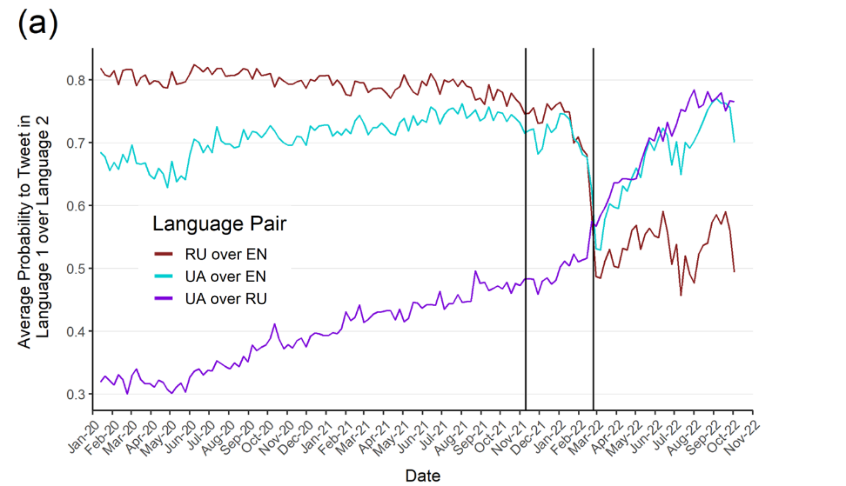
\includegraphics[width=1.0\linewidth]{Figures/ru_ua_twitter.png}
\decoRule
\caption[Ukrainian language dynamics on Twitter]{Tweeting language dynamics in 2020-2022, showing the increasing use of Ukrainian compared to Russian (purple line) throughout the period.}
\label{fig:twitter}
\end{figure}

Notably, of the 1,363 users tweeting predominantly ($>80$\%) in
Russian before the outbreak of the war, 61\% started tweeting in Ukrainian more
after the outbreak, and \textasciitilde25\% (341) started tweeting
\emph{predominantly} in Ukrainian (hard-switch from
Russian to Ukrainian); there were only~3\% UA$\rightarrow$RU hard-switches 
in that period.
The authors interpret switching from Russian to Ukrainian as users\textquotesingle{} conscious
choice towards a more Ukrainian identity.%
\footnote{
% Switching from
%   Russian to Ukrainian, for a habitual Russian speaker who considers Russian their mother tongue, is \emph{hard}.
  \href{https://newlinesmag.com/first-person/mother-tongue-the-story-of-a-ukrainian-language-convert/}{Mother
  Tongue: The Story of a Ukrainian Language Convert - New Lines
  Magazine}~\cite{newlinesmagMotherTongue} is a first-hand account of the emotional and cultural aspects of this shift: for a habitual Russian speaker who considers Russian their mother tongue (which in no way conflicts with a Ukrainian ethnic self-identification), a decision to switch to Ukrainian is not just a linguistic change, and not an easy one. 
  % \enquote{There is a dam where communication used to flow freely, but we now police what’s left, looking for the toxic residue of our mother tongue. We now make political statements where we used to speak from our hearts.}
}
Ukrainian Twitter users are not a representative sample of the Ukrainian
population, but the study is likely indicative of
wider societal trends.

With more people switching to Ukrainian partially or full-time, for
different reasons, the importance of Ukrainian NLP grows
correspondingly.

\section{Ukrainian as a mid-resource
language?}\label{ukrainian-as-a-mid-resource-language}

In the taxonomy of languages based on data availability \cite{inclusion}
(see below), Ukrainian is classified in class 3, ``the rising stars'':
languages with a thriving online cultural community that got an energy
boost from unsupervised pre-training, but was let down by insufficient
efforts in \emph{labeled} data collection. Sample languages from that
group include Indonesian, Cebuano, Afrikaans, and Hebrew. (Russian is in
class 4, English and German are in class 5.)

\begin{figure}[t]
\centering
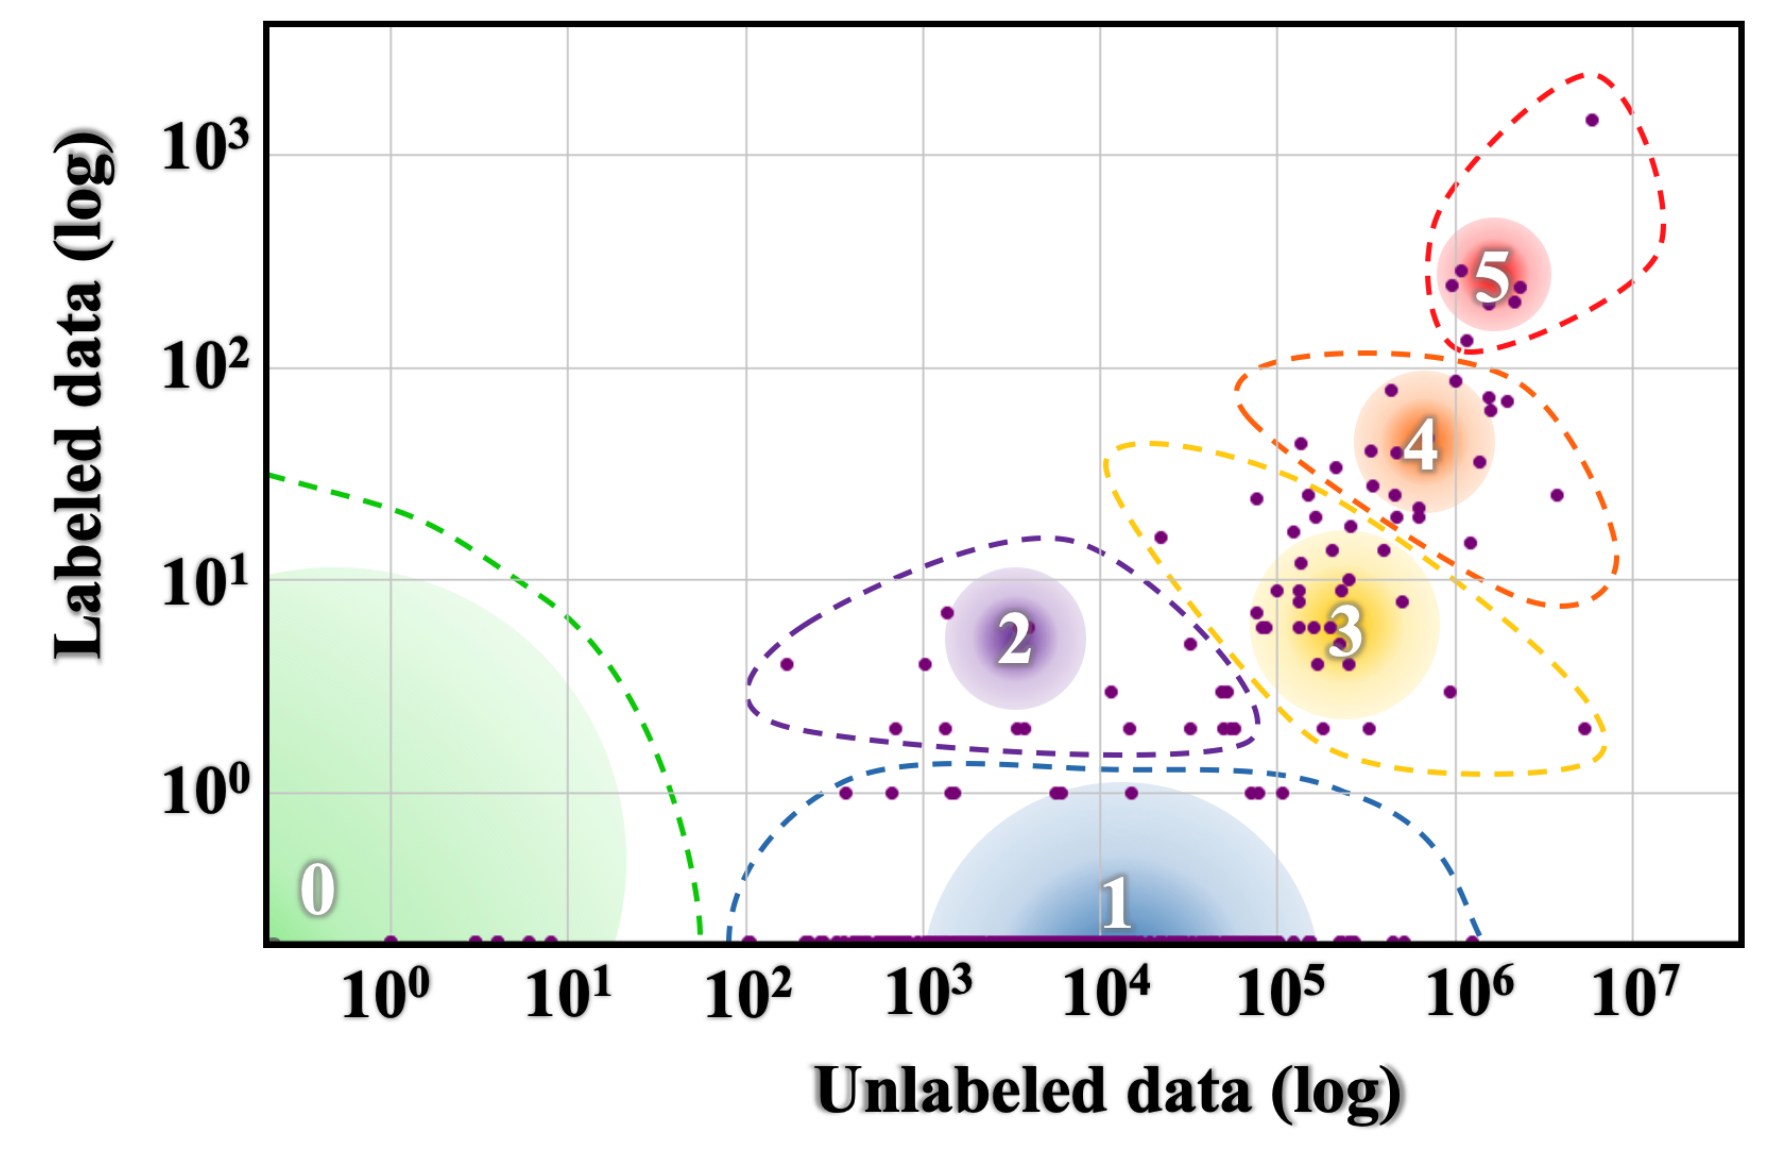
\includegraphics[width=1.0\linewidth]{Figures/Pasted image 20231030165827.png}
\decoRule
\caption[Language resource distribution]{Figure 2 of \cite{inclusion}, showing the language resource distribution. The size of the circle shows the number of languages in that class, the dashed lines show the points covered by that class. Ukrainian belongs to class 3.
% as quoted in \href{https://www.ruder.io/nlp-beyond-english/}{Why You Should Do NLP Beyond English}
}
\label{fig:bender}
\end{figure}

From a different angle, 
% looking at 
in estimates of languages used on the
Internet (as approximated percentages of the top 10M websites), as of
October 2023 Ukrainian is at number 19 (0.6\%), between Arabic and
Greek~\cite{enwiki:1182341232}. English is \#1
(53.0\%), Russian \#3 (4.6\%) and German at \#4 (4.6\% as well).

Ukrainian Wikipedia is 15th by daily views and by number of
articles~\cite{wiki:xxx}.
 
\section{The importance of NLP for mid- and low-resource
languages}\label{the-importance-of-nlp-for-mid--and-low-resource-languages}

\subsection{The Bender rule and language
independence}\label{the-bender-rule-and-language-independence}

Emily M. Bender in 2011~\cite{bender} formulated what would come to be
known as the Bender rule~\cite{benderpost}: ``Name the languages we
study''.

Her original 2011 paper --- written in the pre-LLM era --- discusses the
problem of language independence: the extent to which NLP
research/technology can scale over multiple (or
\textquotesingle all\textquotesingle) languages. In her more recent
writing on the topic, she notes how work on languages other than English
is often considered ``language specific'' and thus viewed as less
important~\cite{benderpost}, and the underlying misconception that
English is a sufficiently representative language and therefore work on
English is not language specific.

An NLP system that works for English is not guaranteed to behave
similarly for other languages, unless explicitly designed and tested for
that. Or in different words, \textbf{``English is Neither Synonymous with
Nor Representative of Natural Language''}~\cite{benderpost}.

She mentions 8 properties of English that highlight
its shortcomings in representing all languages, of them
4 differentiate it from Ukrainian as well: little inflectional morphology, fixed word order,
possible matches to database field names or ontology entries, and
massive amounts of training data available.

\subsection{Russian is neither synonymous nor representative of (East-)Slavic languages}
\label{sec:russian-not-representative}

In the context of this Thesis, an interesting facet of this issue was 
% my intuitive assumption that 
Python\textquotesingle s \texttt{sort()} function sorting letters correctly for English but not for Ukrainian, leading to a bug discovered during human validation.%
% it didn\textquotesingle t.
\footnote{For
details about the sorting issue, see \autoref{valid-lmentry-static-ua} about the
LMentry-static-UA task.} In
hindsight absolutely unsurprising. 
But — for many English-only-speakers many things \emph{just work} and one can't
blame them for assuming that if it works for English, it works for other languages just as well, and more generally that results and approaches
generalize. 
(Even for a native Ukrainian speaker that should have known better this was surprising, illustrating how all-encompassing such world models can be). 

Expanding on that — the Russian alphabet gets sorted correctly by default, except for the very rarely used 
 and grammatically optional letter \textit{Ё} (that ends up at the beginning). 
 It's the same point as above — it's easy to conclude (or, more likely, never even ask the question) that if an approach works for Russian (and in many cases it will), it will work for Ukrainian as well. 
 
The point Emily Bender was making about English, if applied to Russian 
(along with most arguments about why more care in this area is important), leads to interesting insights. 

But there's a larger point to be made here on the relationship between Ukrainian and Russian.
As part of the work on this Thesis, instances of the following were seen:

\begin{enumerate}
    \tightlist
    \item Datasets (or parts of them) labeled as Ukrainian that in reality contained Russian (or a mix of both).
    \item The first result\footnote{\href{https://raw.githubusercontent.com/hermitdave/FrequencyWords/master/content/2016/uk/uk_50k.txt}{https://raw.githubusercontent.com/hermitdave/FrequencyWords/master/content/2016/uk/uk\_50k.txt}} on Github for a list of most frequent Ukrainian words contains \textit{many} Russian ones, to the point that they seem to make up around half of the source material.%
    \footnote{Often higher up than the Ukrainian alternatives: the fifth word is \textit{ты\gl{you}}, the Ukrainian word for \textit{you} is 12th from top. (The Russian word even contains the letter \textit{ы} that doesn't exist in Ukrainian, so some words can be filtered out.) Same for the 4th and 7th. Practically, number 4, 5, 8 are the first unambiguously Russian words. The first unambiguously Ukrainian ones are 7 and 13. I'd estimate that about half of the language used for the list was Russian. The frequencies point to that as well: the first 3 words are common to both Russian and Ukrainian, the first word being the first pronoun \textit{я} (``I''). It can't be the most common word in Ukrainian (and indeed isn't according to other frequency lists), but its position makes sense if one assumes the dictionary sums up the occurrences of Ukrainian and Russian words from the same dataset.
    }
    \item That list was generated based on OpenSubtitles2016~\cite{lison2016opensubtitles2016} corpus data, and such a large amount of Russian words would imply many instances of Russian subtitles incorrectly tagged as Ukrainian; which is not an atypical situation for multilingual corpora (\autoref{sec:multilingual}).
    % FIX TODO add examples from UNLP chat
    \item LLMs generating the story in Russian when explicitly prompted for an Ukrainian one (see \autoref{fig:llama}). LLMs using Russian names for animals, errors in (grammatical) gender agreement for the animals whose (grammatical) gender is different in Ukrainian and Russian.
\end{enumerate}

\begin{figure}[t]
\centering
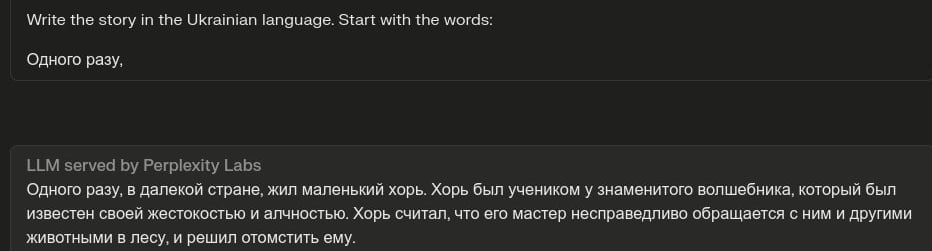
\includegraphics[width=1.0\linewidth]{Figures/llama.jpg}
\decoRule
\caption[llama2-70b-chat generating a Russian story instead of an Ukrainian one]{llama2-70b-chat generating a story that starts the with two Ukrainian words specified in the prompt and 
switches to Russian immediately afterwards.}
\label{fig:llama}
\end{figure}

The historical background described in \autoref{sec:ukr-lang-history} serves chiefly to illustrate the extent to which the Ukrainian language's existence has been threatened.

% Much more recently, 3 April 2022,
% %(same day as the bodies of Russian civilians were discovered in Bucha), 
% Russian state-owned agency RIA Novosti published 
% an article~\cite{sergeytsev2022russia} 
% entitled ``What Russia should do with Ukraine''%
% \footnote{A translation of the article to English: \href{https://medium.com/@kravchenko_mm/what-should-russia-do-with-ukraine-translation-of-a-propaganda-article-by-a-russian-journalist-a3e92e3cb64}{https://medium.com/@kravchenko\_mm/what-should-russia-do-with-ukraine-translation-of-a-propaganda-article-by-a-russian-journalist-a3e92e3cb64}.
% To the extent that the presence of a Wikipedia page can be considered a proxy for notability, the article has a Wikipedia page translated to 16 languages:
% \href{https://en.wikipedia.org/wiki/What_Russia_Should_Do_with_Ukraine}{https://en.wikipedia.org/wiki/What\_Russia\_Should\_Do\_with\_Ukraine}.
% },
% where it called for the full destruction of Ukraine as a state, of the Ukrainian national identity (\textit{de-ukrainisation}), and the integration of its population into "Russian Civilisation", 
% and has been called an incitement to genocide in German\footnote{\href{https://www.tagesspiegel.de/politik/ria-novosti-ruft-zur-vernichtung-der-ukraine-auf-5139691.html}{https://www.tagesspiegel.de/politik/ria-novosti-ruft-zur-vernichtung-der-ukraine-auf-5139691.html}} and international media.

And LLMs switching to Russian or using Russian words and sentences inside Ukrainian language, or the same happening in a text-to-speech conversation, or having to switch to Russian just to make a system functional --- in light of that context, 
these scenarios are more significant than mere annoyances for many Ukrainians.%
\footnote{The lack of Ukrainian language support in Apple Siri is representative here, with a petition (\href{https://www.change.org/p/apple-teach-siri-to-understand-ukrainian-language}{https://www.change.org/p/apple-teach-siri-to-understand-ukrainian-language}), the many requests for Ukrainian language support on their community forum (\href{https://discussions.apple.com/search?q=siri+Ukrainian}{https://discussions.apple.com/search?q=siri+Ukrainian}) and elsewhere 
(\textit{\enquote{because of the war in Ukraine I cannot (do not want to) use Siri in russian anymore}}: \href{https://www.reddit.com/r/MacOS/comments/tejp3z/siri_in_ukrainian_language/}{https://www.reddit.com/r/MacOS/comments/tejp3z/siri\_in\_ukrainian\_language/}).
} 
% it's clear why for many Ukrainians these are more than simply a nuisance. 
(In fact, they were a powerful motivator for the Eval-UA-tion volunteer human annotators in the Telegram chat: many had their own experiences to share on the matter, and helping with a Ukrainian LLM benchmark was one actionable way to change this status quo.)

\section{Roadmap}\label{roadmap}

This Thesis tackles the following problems:

\begin{enumerate}
\tightlist
    \item Describe modern Ukrainian NLP, including the availability of corpora, datasets, and resources.
    \item Create novel Ukrainian-language datasets usable as benchmark tasks for evaluating Large Language Models.
    \begin{enumerate}
        \item create human baselines for all of the newly-established datasets
        \item make the datasets available and easily accessible through an established platform
    \end{enumerate}
    \item Evaluate both open and commercial LLMs on these datasets.
\end{enumerate}



% \begin{itemize}
% \tightlist
% \item
%   Evaluate whether cross/multi language models that include Ukrainian
%   perform equally well to Ukrainian monolingual models
% \item
%   Research whether there\textquotesingle s a significant difference in
%   scores of tasks translated to Ukrainian using automated methods as
%   opposed to human translations
% \item
%   Compare the extent to which the language matters when solving
%   problems, with the following languages:

%   \begin{itemize}
%   \tightlist
%   \item
%     Ukrainian
%   \item
%     English (high resource language)
%   \item
%     Russian (high resource language from the same language family as
%     Ukrainian)
%   \end{itemize}
% \end{itemize}